\section{Results}\label{sec:results}
\subsection{Descriptive Statistics}\label{subsec:data_exam}

\begin{table}[H]
    \centering
    \begin{tabular}{lccccc}
        \toprule
        \textbf{Variable} & \textbf{N} & \textbf{Mean} & \textbf{SD} & \textbf{Min} & \textbf{Max} \\
        \midrule
        $growth$ & 120 & 2.40 & 3.07 & -6.70 & 9.30 \\
        $vol$ & 120 & 0.31 & 0.22 & 0.01 & 0.99 \\
        $trade$ & 120 & 51.60 & 26.19 & 23.56 & 100.82 \\
        $gfcf$ & 120 & 23.28 & 3.39 & 16.44 & 37.29 \\
        $hicp$ & 120 & 3.33 & 3.38 & -1.10 & 17.00 \\
        $govexp$ & 120 & 45.91 & 5.65 & 33.50 & 57.90 \\
        \bottomrule
    \end{tabular}
    \caption{Descriptive statistics for the estimation sample}
    \label{tab:descriptive}
\end{table}

The table \ref{tab:descriptive} presents the summary statistics for the estimation sample of 120 country and year observation.
The range of the exchange rate volatility which runs from 0.01 to 0.99 percentage measured as the annual mean of daily conditional standard deviations.
The lower end belongs to Denmark with its highest annual over the twenty year at 0.029.
It is still around ten times smaller than the average for any other currency in the sample.
This is the ERM II mechanism peg described before.
And the upper end belongs to the freely floating currencies in crisis years.

\vspace{\baselineskip}

The spread of trade intensity also stand out.
The standard deviation of 26.19 is half of its mean at 51.6 which is unusually large for macroeconomic variables.
This shows in the differences between countries instead of the movement over time.
The range from from 23.56 to 100.82 percentage of GDP runs from Denmark and Sweden at the lower end to Czech Republic and Hungry at the upper end.
It shows above one hundred percentage are not error. 
Trade counts the full value of goods crossing border which GDP counts only the value added at domestic so a country that import parts and re-export the assembled product count the same value twice in the trade.

\vspace{\baselineskip}

Growth ranges from -6.70 to 9.30 percentage with the negative end reflecting the recessions of 2009 and 2020.
Inflation ranges from -1.1 to 17 percentage covering both falling prices and the high inflation years of the late 2000s and 2020.


\begin{table}[H]
    \centering
    \begin{tabular}{lcc}
        \toprule
        \textbf{variable} & \textbf{centered} & \textbf{raw}\\
        \midrule
        $vol$                  &      1.25 &  5.91\\
        $trade$                &      1.19  & 4.75\\
        $vol x trade$          &      1.37  & 12.28\\
        $gfcf$                 &      1.25  & 1.25\\
        $hicp$                 &      1.34  & 1.34\\
        $govexp$               &      1.42  & 1.42\\
        \bottomrule
    \end{tabular}
    \caption{Variance inflation factors for the regressors.}
    \label{tab:vif}
\end{table}

Table \ref{tab:vif} presents variance inflation factors for estimated model and comparison for the same model with volatility and trade intensity on their original form.
In the estimated specification every factor ranges between 1.19 to 1.42 below the threshold of ten at which collinearity is usually a problem.
With the level below the threshold the regressors and coefficients can be read individually.

\vspace{\baselineskip}

The original form shows different result. Volatility, trade intensity and interaction rises to 5.91, 4.75 and 12.28 respectively.
The three controls remain unchanged since shifting a variable by a constant does not change its relationship to others.
Only the product is affected and with its two variables.
Nothing with the data is changed but only the point the variables are measured from.
Trade intensity multiplying volatility always means multiplying a large number.
The product is close to volatility scaled up by constants.
Two move together which is what VIF measures.
By centreing both variables on their own means and product no longer tracks volatility.
The high VIF number reflects where the variables are measured.
Since both versions produce identical coefficients, standard errors and residuals so the centred variables are the one matter.

\vspace{\baselineskip}

The correlations between variables do not exceeds 0.36 in absolute value (See Appendix~\ref{appendA} for further details).
The correlation between volatility and inflation is 0.29 so nominal exchange rate movement carries some inflation instability.
The correlation between volatility and growth is -0.08 close to zero which is what makes the conditional specification necessary.

\begin{figure}[H]
\label{fig:garchvol}
    \centering
    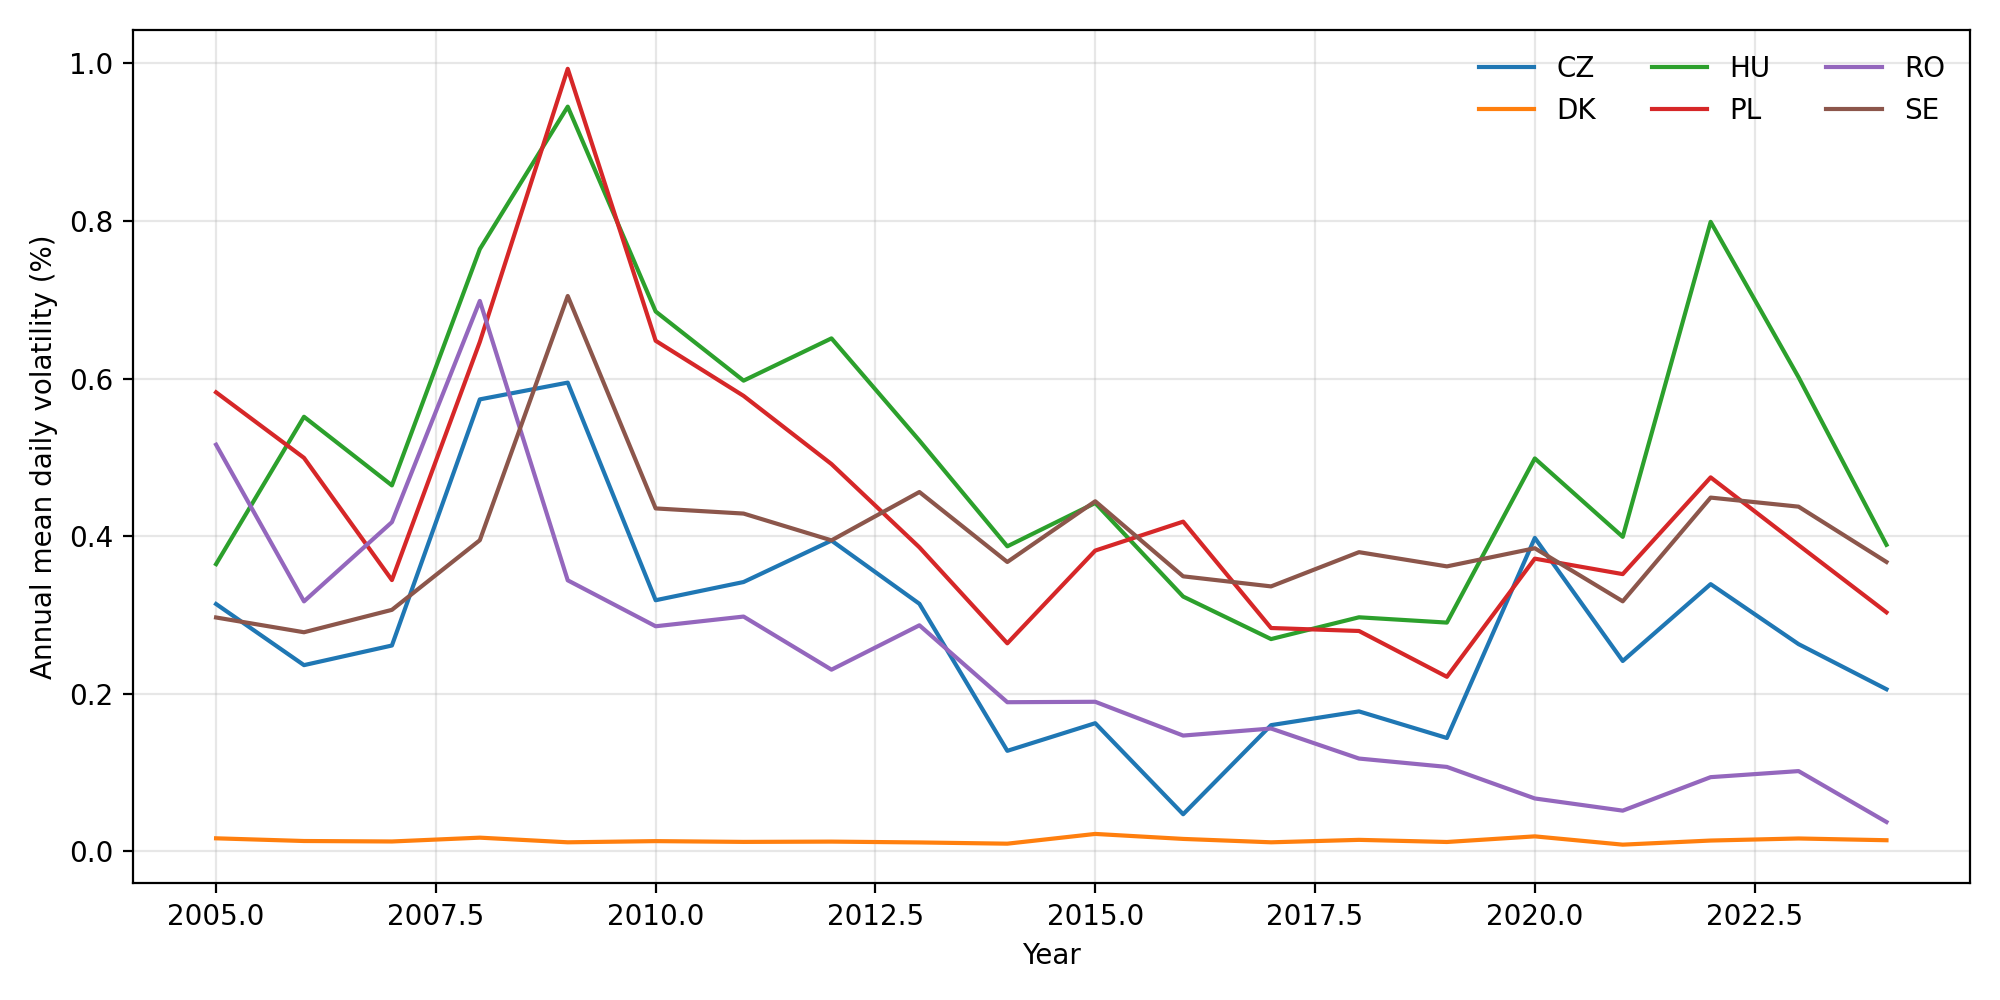
\includegraphics[width=0.75\textwidth]{fig/volatility.png}
    \caption{Annual Mean Conditional Volatility from GARCH(1,1)}
\end{figure}

Figure~\ref{fig:garchvol} presents the annual mean conditional volatility of each currency against the euro obtained from the GARCH(1,1).
As we expected the Danish Krone never rises above 0.03 in any year in the sample while other five currencies average between 0.26 to 0.52.
This the ERM II arrangement we discussed before.
The Danish Krone is held close to its central rate so there is very little movement for the model to measure.
GARCH describes how volatility changes over time and know Danish Krone barely moves.
The Danish Krone fit runs against the model's parameter limits.
This figure still measure how much the currency moved but the only record that the peg held instead of how volatility behaved.

\vspace{\baselineskip}

The clearest thing we can see from this figure is the fluctuation in 2009.
Volatility rises sharply in all five currencies peaking at 0.99 for the Polish zloty.
Both of the movement are more than double their sample averages.
This is exactly showing the global financial crisis and its the largest movement in the twenty years.
We can also see the other features from this figure.
The 2020 shock is much smaller than 2009 its volatility rises in that year but only to around 0.4 to 0.5.
And the second highest reading in the sample is not a crisis where the Hungarian forint reaches 0.8 in 2022 during European inflation.

\vspace{\baselineskip}

We can also spot different pattern in Czech koruna between 2013 to 2017.
It falls to 0.05 in 2016 the lowest recorded by any floating currency in the sample and recovers after 2017.
This is the Czech National Bank's exchange rate floor we mentioned and its effect on the estimation (See Appendix~\ref{appendB} for further details).
The koruna during this period is not a floating currency but interrupted as managed one.


\subsection{Regression Results}\label{subsec:panel}


\begin{table}[H]
    \centering
    \small
    \begin{tabular}{lccc}
        \toprule
        \textbf{Explanatory variable} & \textbf{Model 1} & \textbf{Model 2} & \textbf{Model 3} \\
        \midrule
        $vol$            & $-1.396$   & $-4.255$*** & $3.691$ \\
                              & $(1.443)$  & $(1.406)$         & $(2.331)$ \\[2pt]
       $trade$       & $0.000$    & $0.068$           & $0.051$* \\
                              & $(0.007)$  & $(0.082)$         & $(0.028)$ \\[2pt]
        $vol x trade$ & $-0.076$ & $-0.047$        & $-0.096$** \\
                              & $(0.061)$  & $(0.052)$         & $(0.048)$ \\[2pt]
        $gfcf$                  & $-0.007$   & $0.345$** & $0.263$*** \\
                              & $(0.098)$  & $(0.159)$         & $(0.085)$ \\[2pt]
        $hicp$                  & $-0.013$   & $-0.044$          & $-0.195$** \\
                              & $(0.090)$  & $(0.110)$         & $(0.092)$ \\[2pt]
        $govexp$ & $-0.169$*** & $-0.407$** & $0.019$ \\
                              & $(0.050)$  & $(0.194)$         & $(0.090)$ \\
        \midrule
        Country fixed effects & No  & Yes & Yes \\
        Year fixed effects    & No  & No  & Yes \\
        Observations          & 120 & 120 & 120 \\
        Number of countries   & 6   & 6   & 6 \\
        $R^2$                 & 0.151 & 0.347 & 0.787 \\
        Wald test & $F(6,113) = 3.337^{***}$ & $F(11,108) = 5.222^{***}$ & $F(30,89) = 10.962^{***}$ \\
        \bottomrule
    \end{tabular}
    \caption{Panel regression results. Driscoll--Kraay standard errors in
    parentheses. *** $p<0.01$, ** $p<0.05$, * $p<0.1$.}
    \label{tab:panel_results}
\end{table}

The table \ref{tab:panel_results} presents the regression under three specifications.
The first model pooled all 120 observations and treats them as one population.
The second model put in country as dummy variable.
The third model put in country and year together as dummy variables.
The standard errors are Driscoll-Kraay for this table.
We also computed the p-values under ordinary, Newey-West and cluster robust estimators (See Appendix \ref{appendC} for further details).
The estimates change very differently between specifications.
It is worth explaining the result since it determines which specification to use.

\vspace{\baselineskip}

The model 1 uses stacked panel of 120 country year rows and without fixed effects.
It shows nothing is significant except government expenditure.
The R-square shows 15 percentage which means only little variation in growth is explained by the model.
It is showing a poor fit and it is expected from this specification.
Because Denmark and Romania are very different economics and pooling them together means the model must explain the difference between a Danish year and a Romanian year using only six variables in the regression.
Most of the difference comes from things the model does not measure.

\vspace{\baselineskip}

The model 2 puts country fixed effect for stacked panel.
It is giving each country its own intercept as dummy variable and remove the problem.
This model no longer has to explain why Denmark grow differently from Romania on average.
It only has to explain why each country grows differently from its own average in given year.
The model fit improves to 35 percentage.
The volatility becomes significant with coefficient of -4.255.
It is saying that a country grows slowly in years when its currency is more volatile.
The country fixed effects model still cannot explain for what happened to all six countries in the same year.
The model 3 adding year effects with country effect changes the result.
Volatility loses its significance and coefficient changes to 3.691.
The interaction between volatility and trade intensity becomes negative at -0.096 and significant at the 5 percentage.
This model fits rises to 78.7 percentage.

\vspace{\baselineskip}

The coefficient on volatility changes sign between the two models which requires explanation.
The country fixed effects model compares each country with itself over time which removes everything fixed about the country itself.
Country effects cannot remove anything that hit all six countries in the same time which is the financial crisis.
In 2009 exchange rate volatility rose in every floating currency in the sample and output fell in every country.
The model observes high volatility and low growth and presents a negative relationship between them.
But the volatility and growth did not cause each other.
Both of them were consequences of the crisis and the model without the year fixed effect cannot tell the difference.

\vspace{\baselineskip}

Year effects solve this by giving each year its own intercept.
The 2009 crisis is now absorbed by the year effect so it can no longer show up in the volatility coefficient.
What it remains is the comparison whether a country whose currency was unusually volatile in a given year grew differently from one whose currency was not.
This comparison gives a different answer from the country fixed effects model and it is the one this thesis relies on.
So the model with both country fixed and year fixed specification is preferred for the rest of the analysis.

\vspace{\baselineskip}
The three control variables behave differently across the specifications and the pattern is informative.
Gross fixed capital formation is positive and significant under both fixed effects specifications at 0.345 and 0.263.
This is expected result where countries invest more in years when they grow more and two move together.
Inflation is significant only in the both fixed effects specification at -0.195.
Higher inflation goes with slower growth but only once year effects are included.
Before that inflation and growth were both moving with common cycle and the model could not separate the two.
Government expenditure shows in other way. 
It is significant in the first two models but not the third.
This suggests what looked like an effect was really the common cycle instead of specific to individual countries.
Adding year effects removes it.
A final point on how the volatility coefficient should be read.
The coefficient on volatility in the both fixed effects specification is not the effect of volatility in general.
Because volatility and trade intensity are centred.
It gives the effect for country with average euro area trade exposure.
It does not explain what happens at higher or lower levels of exposure.


\subsubsection{Joint Significance of Coefficients}\label{joint_sign}
\begin{table}[H]
    \centering
    \small
    \setlength{\tabcolsep}{5pt}
    \begin{tabular}{llccc}
        \toprule
        \textbf{Specification} & &
        \textbf{No} & \textbf{No} & \textbf{Without both} \\
        & & \textbf{trade exposure} & \textbf{volatility} & \textbf{variables} \\
        \midrule
        Model 1 & F  & 0.768     & 0.738     & 0.566 \\
                   & df & (2,\,113) & (2,\,113) & (3,\,113) \\
                   & p  & 0.466     & 0.481     & 0.638 \\
        \midrule
        Model 2 & F  & 1.686       & 4.644       & 5.328   \\
                   & df & (2,\,108) & (2,\,108) & (3,\,108) \\
                   & p  & 0.19       & 0.0116       & 0.0018   \\
        \midrule
        Model 3 & F  & 4.721     & 2.064       & 4.003 \\
                   & df & (2,\,89)  & (2,\,89)  & (3,\,89) \\
                   & p  & 0.011     & 0.133       & 0.010 \\
        \bottomrule
    \end{tabular}
    \caption{Wald tests of joint restrictions, computed from the Driscoll--Kraay
    covariance matrix.}
    \label{tab:wald}
\end{table}

The volatility and trade intensity each appear twice in the model as their own and inside the interaction.
Whether a variable matter is a claim about two coefficients together.
Testing them one at a time can miss a relationship since coefficients estimated together are not independent.
Table \ref{tab:wald} presents Wald tests for three restrictions computed from the Driscoll-Kraay covariance matrix.

\vspace{\baselineskip}

In model 1 presents no rejection. The three restrictions p-value are 0.466, 0.481 and 0.638.
It shows they are jointly insignificant. 
This matches the coefficient table where only government expenditure was significant.
The model 2 rejects volatility at p=0.012 and trade exposure fails to reject at p=0.19.
This pattern reverses in model 3.
It rejects trade exposure at p=0.011 and fails to reject volatility at p=0.133.
This explains what happened to the coefficient.
Without year fixed effect the model reads the 2009 crisis as an effect of volatility so volatility looks significant on its own.
When the movement is absorbed by the year effects and it becomes insignificant.
So the trade exposure remains significant and shows how much the effect of volatility depends on a country's trade with the euro area.

\vspace{\baselineskip}

In the model 3 which we focusing on the volatility and its interaction are jointly insignificant at p=0.133.
There is no evidence that volatility affects growth independently of trade exposure.
Trade exposure rejects at p=0.011 and it is stronger evidence than the interaction coefficient alone.
The coefficient is significant at p=0.046 close to the threshold that it moves depending on the covariance estimator.
The joint test also does not depend on whether the variables are centred.

\subsubsection{Marginal Effect of Volatility}\label{sec:mar_eff_vol}

\begin{figure}[H]
\label{fig:marg_eff}
    \centering
    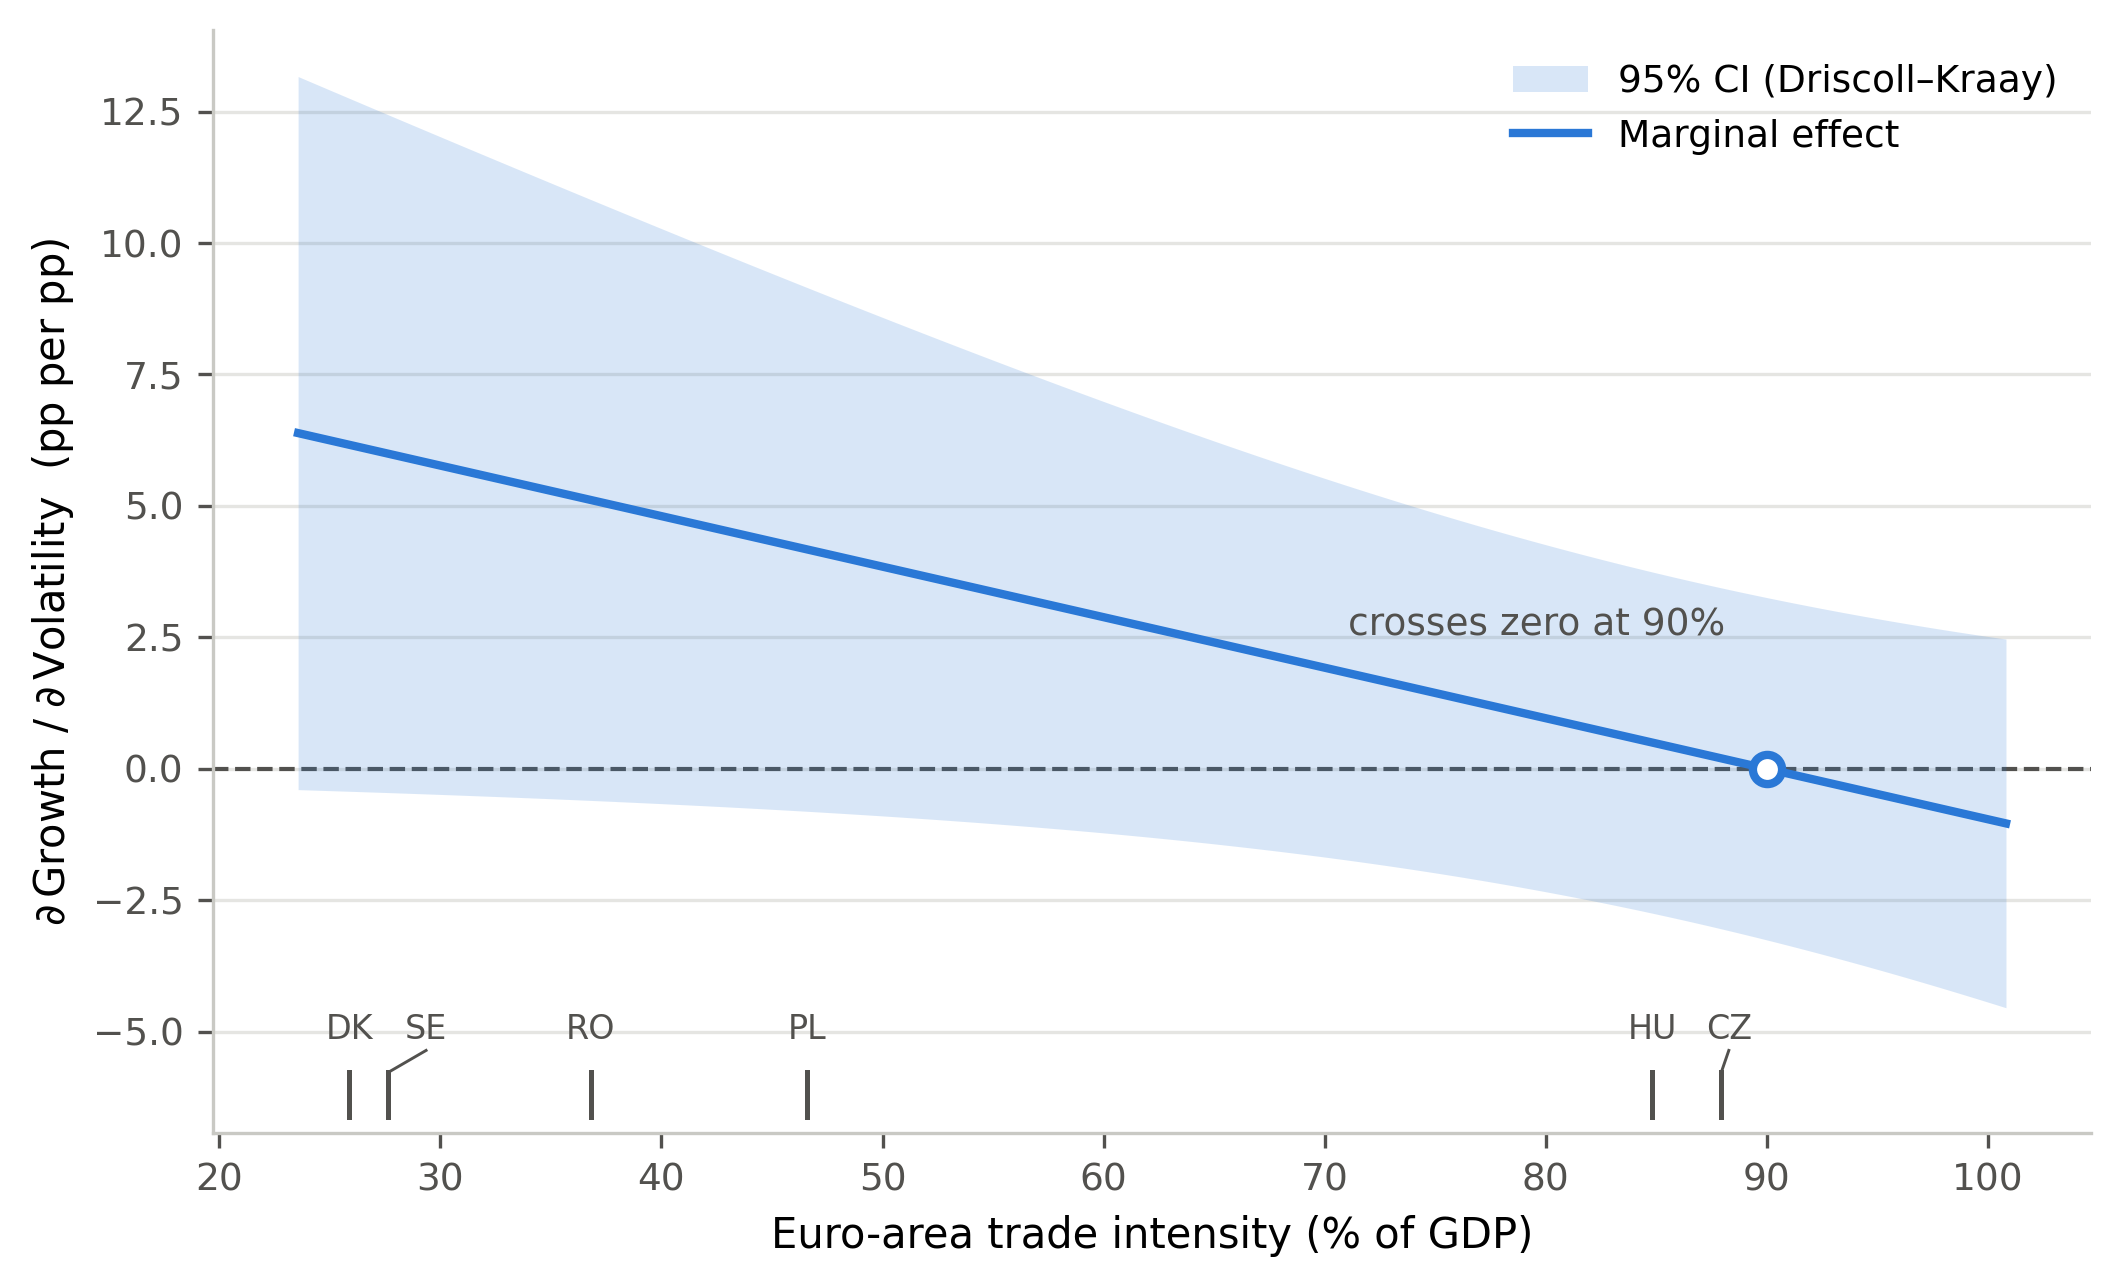
\includegraphics[width=0.75\textwidth]{fig/marginal_effect.png}
    \caption{Marginal effect of volatility on growth by euro area trade intensity with 95\% confidence intervals}
\end{figure}

The joint tests we discussed shows that trade exposure matters but no explanation.
Because the model contain an interaction.
The effect of volatility is not a single number which it changes with a country's trade exposure to the euro area.
This figure \ref{fig:marg_eff} presents the marginal effect of volatility on growth where the line slopes downward across the whole range.
Denmark and Sweden at the left end at around 26 percentage of GDP.
The estimated effect of volatility on growth is positive around 6.3 points.
It fails to 1.1 points by the time trade intensity is near 79 percentage and crosses zero at 90 percentage.
Hungary and the Czech Republic at 85 and 88 percentage respectively.
The shape is expected where a country trade little with the euro area and a moving currency mostly absorbs shocks and the relationship with growth is positive.
The trade increases when the cost volatility imposes on trade grows and offsets the benefit.

\vspace{\baselineskip}

The shaded band includes zero where every point across the range.
The confidence interval covers both positive and negative values.
The lowest p value at 0.066 (See Appendix \ref{appendD} for further details).
This means the negative slope cannot be separated from a flat line at zero.
The pattern matches what the theory predicts.

\vspace{\baselineskip}

It is wider for band at both ends.
The 25 percentage trade intensity runs from -1 to +13 and -4.5 to +2.5 at 100 percentage.
The reason is the marginal effect depends on the interaction coefficient multiplied by the distance from the mean.
The further from the mean the more coefficient's uncertainty carries through.
The largest estimated effects at the ends of the range which is unreliable for the estimates.

\vspace{\baselineskip}
The figure shows no observations in the middle.


\subsection{Diagnostic}\label{subsec:diagnostic}
Jarque-Bera      stat=  53.78  p=0.0000   skew=-0.491  excess kurtosis=+3.129
   H0: normal residuals. Rejection does NOT threaten consistency or unbiasedness
   of the slopes -- only the exact small-sample t and F distributions, which the
   Driscoll-Kraay standard errors replace anyway. Expected with macro data.

\vspace{\baselineskip}

Breusch-Pagan    stat=  39.15  p=0.1224
   H0: constant error variance. Rejection would mean OLS standard errors are
   wrong; the robust estimators already handle it.

\vspace{\baselineskip}

Ramsey RESET 2   F=  0.004  p=0.9479
Ramsey RESET 3   F=  0.722  p=0.4887
   H0: no omitted non-linearity. This is the one test where NON-rejection is the
   good outcome rejection would say the functional form itself is wrong.

\vspace{\baselineskip}

Within-country AR(1)   rho=+0.1446  p=0.1177  n=114
   H0: no first-order serial correlation in the residuals. Significant rho would
   mean the Driscoll-Kraay lag truncation (maxlags=2) is too short.
   Verdict: no evidence of serial correlation.



\subsection{Robustness}\label{sec:robustness}

\begin{table}[H]
    \centering
    \begin{tabular}{lcccc}
        \toprule
        \textbf{Variable} & \textbf{sd\_between} & \textbf{sd\_within} & \textbf{ratio} \\
        \midrule
        vol\_c & 0.179 & 0.140 & 1.278 \\
        trade\_c & 27.941 & 5.466 & 5.112 \\
        vol\_x\_trade & 4.309 & 3.582 & 1.203 \\
        gfcf\_pct\_gdp & 2.692 & 2.319 & 1.161 \\
        hicp & 1.275 & 3.172 & 0.402 \\
        gov\_exp\_pct\_gdp & 5.617 & 2.324 & 2.417 \\
    \end{tabular}
    \caption{Cross-sectional Variation}
    \label{tab:var}
\end{table}

\begin{table}[H]
    \centering
    \begin{tabular}{lccc}
        \toprule
        \textbf{Variable} & \textbf{GARCH} & \textbf{TGARCH} & \textbf{GARCH,No GFCF}\\
        \midrule
        Volatility & +3.691 (p = 0.117) & +3.657 (p = 0.115) & $+5.6159$(p = 0.038)\\
        Trade intensity & +0.051 (p = 0.071) & +0.052 (p = 0.066) & $+0.0227$ (p=0.516)\\
        Volatility × trade & $-0.096$ (p = 0.046) & $-0.093$ (p = 0.051) & $-0.1384$(p=0.029)\\

    \end{tabular}
    \caption{Two-way fixed effects, Driscoll–Kraay standard errors, N = 120. Regression coefficients (standard errors omitted).}
    \label{tab:two_way}
\end{table}

\begin{sidewaystable}
    \centering
    \sisetup{table-number-alignment=center}
    \begin{tabular}{l
                    S[table-format=3.0]
                    S[table-format=-1.4] S[table-format=1.4]
                    S[table-format=-1.4] S[table-format=1.4]
                    S[table-format=-1.4] S[table-format=1.4]
                    S[table-format=2.4]  S[table-format=1.4]}
        \toprule
        & & \multicolumn{2}{c}{Volatility}
          & \multicolumn{2}{c}{Trade intensity}
          & \multicolumn{2}{c}{Volatility $\times$ trade}
          & \multicolumn{2}{c}{Joint test} \\
        \cmidrule(lr){3-4} \cmidrule(lr){5-6} \cmidrule(lr){7-8} \cmidrule(lr){9-10}
        \textbf{Sample} & {\textbf{N}}
        & {Coef.} & {$p$} & {Coef.} & {$p$} & {Coef.} & {$p$} & {$F$} & {$p$} \\
        \midrule
        Full sample                & 120 &  3.6911 & 0.1168 &  0.0510 & 0.0709 & -0.0961 & 0.0462 &  4.7214 & 0.0113 \\
        Excl. DKK (pegged)         & 100 &  3.6796 & 0.2702 &  0.0519 & 0.0149 & -0.0961 & 0.0818 & 13.7952 & 0.0000 \\
        Excl. crisis (2008--09, 2020) & 102 & -0.3114 & 0.8361 &  0.0528 & 0.1512 &  0.0016 & 0.9713 &  1.0778 & 0.3456 \\
        2010--2024 only            &  90 & -2.2944 & 0.2290 &  0.1045 & 0.0011 &  0.0101 & 0.8484 &  5.8781 & 0.0045 \\
        Excl. COVID (2020--21)     & 108 &  4.3601 & 0.0561 &  0.0662 & 0.0268 & -0.0940 & 0.0443 &  5.3945 & 0.0064 \\
        \midrule
        \multicolumn{10}{l}{\emph{Leave-one-country-out}} \\
        \quad Drop CZ              & 100 &  5.3779 & 0.0163 &  0.0931 & 0.0015 & -0.1417 & 0.0040 & 10.1541 & 0.0001 \\
        \quad Drop DK              & 100 &  3.6796 & 0.2702 &  0.0519 & 0.0149 & -0.0961 & 0.0818 & 13.7952 & 0.0000 \\
        \quad Drop HU              & 100 &  3.9802 & 0.1442 & -0.0170 & 0.6048 & -0.1355 & 0.0105 &  3.9792 & 0.0231 \\
        \quad Drop PL              & 100 &  2.8943 & 0.1686 &  0.0295 & 0.3591 & -0.0691 & 0.2076 &  1.9993 & 0.1431 \\
        \quad Drop RO              & 100 &  1.0950 & 0.6699 &  0.0731 & 0.0714 & -0.0673 & 0.1703 &  2.1701 & 0.1218 \\
        \quad Drop SE              & 100 &  4.4230 & 0.0676 &  0.0480 & 0.1780 & -0.1043 & 0.0339 &  3.4291 & 0.0380 \\
        \bottomrule
    \end{tabular}
    \caption{Robustness checks. Two-way fixed effects re-estimated on subsamples,
    Driscoll--Kraay standard errors. Coefficients are reported for centred volatility,
    centred trade intensity and their interaction; centring is held at the full-sample
    origin so the main effects stay comparable across rows. The joint test is a Wald
    $F$ test of $\beta_{\text{trade}} = \beta_{\text{vol} \times \text{trade}} = 0$
    under the Driscoll--Kraay covariance. Since Denmark is the pegged currency, the
    rows \emph{Excl.\ DKK} and \emph{Drop DK} are the same subsample.}
    \label{tab:robust}
\end{sidewaystable}

% The rotated table is a float and cannot be pinned with [H]. Without this barrier
% it drifts past the end of the section and the conclusion is typeset ahead of it.
\FloatBarrier
